\section{Results}
\label{sec:results}

The following subsections present computational results obtained from the 
implementations of the CWS algorithm, 2-opt local search and SA procedures 
described over Sections~\ref{sec:intro} and~\ref{sec:method}.\vertbreak

The tests were performed on a 64-bit machine equipped with a Intel(R) Core(TM) 
i5-3320M CPU (2 cores), with a clock rate of 2.60\,GHz, 5.7 GB of RAM.

\subsection{CWS and 2-Opt Local Search Combination}
\label{subsec:res-cws}

Tables~\ref{tab:results-1} to~\ref{tab:results-3} provide a list of the 
results obtained by the proposed implementation(s), against several 
datasets available in~\cite{website:cvrp-datasets}. For each dataset, we provide 
results for (1) the parallel version of the CWS, (2) the implemented sequential 
version of the CWS and (3) the enhancements (if any) provided by the implemented 
local search routine. Table~\ref{tab:results-1} provides a comparison of the 
total cost of the different $N$ routes, while Table~\ref{tab:results-2} compares 
the computation time along the same categories as those present in 
Table~\ref{tab:results-1}. Table~\ref{tab:results-3} compares the number of 
generated routes (for both parallel and sequential versions of the CWS 
algorithm) with the optimal values provided in the 
datasets~\cite{website:cvrp-datasets}\vertbreak

\begin{table}[h!]
    \centering
    \begin{threeparttable}
    \footnotesize
        \begin{tabularx}{0.40\textwidth}{ X X X X }
            %\hline
            \toprule
            \textbf{Dataset} & \textbf{CWS} & \textbf{2-Opt} & \textbf{Optimal} \\ [0.5ex]
            \midrule
            \multirow{2}{*}{A-n32-k5}   & 865\tnote{1}   & 863\tnote{1}   & \multirow{2}{*}{784}  \\ [0.5ex]
                                        & 987\tnote{2}   & 968\tnote{2}   &                       \\ [0.5ex]
            \midrule
            \multirow{2}{*}{A-n34-k5}   & 826   & 809   & \multirow{2}{*}{778}  \\ [0.5ex]
                                        & 990   & 955   &                       \\ [0.5ex]
            \midrule
            \multirow{2}{*}{A-n38-k5}   & 816   & 785   & \multirow{2}{*}{730}  \\ [0.5ex]
                                        & 939   & 908   &                       \\ [0.5ex]
            \midrule
            \multirow{2}{*}{A-n39-k5}   & 925   & 919   & \multirow{2}{*}{822}  \\ [0.5ex]
                                        & 1033  & 1003  &                       \\ [0.5ex]
            \midrule
            \multirow{2}{*}{A-n54-k7}   & 1247  & 1230  & \multirow{2}{*}{1167} \\ [0.5ex]
                                        & 1402  & 1372  &                       \\ [0.5ex]
            \midrule
            \multirow{2}{*}{A-n60-k9}   & 1429  & 1422  & \multirow{2}{*}{1354} \\ [0.5ex]
                                        & 1871  & 1765  &                       \\ [0.5ex]
            \midrule
            \multirow{2}{*}{F-n135-k7}  & 1269  & 1252  & \multirow{2}{*}{1162} \\ [0.5ex]
                                        & 1658  & 1531  &                       \\ [0.5ex]
            \midrule
            \multirow{2}{*}{M-n151-k12} & 1209  & 1198  & \multirow{2}{*}{1053} \\ [0.5ex]
                                        & 1432  & 1404  &                       \\ [0.5ex]
            \midrule
            \multirow{2}{*}{M-n200-k17} & 1504  & 1500  & \multirow{2}{*}{1373} \\ [0.5ex]
                                        & 1865  & 1797  &                       \\ [0.5ex]
            \bottomrule
        \end{tabularx}
        \begin{tablenotes}
            \footnotesize
            \item[1]Parallel version of the CWS algorithm.
            \item[2]Sequential version of the CWS algorithm.
            %\item[3]Enhancements on the solution value provided by [parallel\slash sequential] version.
        \end{tablenotes}
    \caption{Results obtained by the proposed implementation(s) (in terms of 
            total route costs), against several datasets available 
            in~\cite{website:cvrp-datasets}.}
    \label{tab:results-1}
    \end{threeparttable}
    %\end{center}
\end{table}

\begin{table}[h!]
    \centering
    \begin{threeparttable}
    \footnotesize
        \begin{tabularx}{0.40\textwidth}{ X X X }
            %\hline
            \toprule
            \textbf{Dataset} & \textbf{CWS} & \textbf{2-Opt} \\ [0.5ex]
            \midrule
            \multirow{2}{*}{A-n32-k5}   & 0.098\tnote{1}   & 0.007\tnote{1} \\ [0.5ex]
                                        & 0.120\tnote{2}   & 0.011\tnote{2} \\ [0.5ex]
            \midrule
            \multirow{2}{*}{A-n34-k5}   & 0.233 & 0.022  \\ [0.5ex]
                                        & 0.441 & 0.022  \\ [0.5ex]
            \midrule
            \multirow{2}{*}{A-n38-k5}   & 0.321 & 0.024  \\ [0.5ex]
                                        & 0.592 & 0.026  \\ [0.5ex]
            \midrule
            \multirow{2}{*}{A-n39-k5}   & 0.412 & 0.028  \\ [0.5ex]
                                        & 0.692 & 0.028  \\ [0.5ex]
            \midrule
            \multirow{2}{*}{A-n54-k7}   & 0.647 & 0.019  \\ [0.5ex]
                                        & 1.583 & 0.038  \\ [0.5ex]
            \midrule
            \multirow{2}{*}{A-n60-k9}   & 0.818 & 0.033 \\ [0.5ex]
                                        & 2.115 & 0.038  \\ [0.5ex]
            \midrule
            \multirow{2}{*}{F-n135-k7}  & 10.805 & 0.082    \\ [0.5ex]
                                        & 16.313 & 0.091    \\ [0.5ex]
            \midrule
            \multirow{2}{*}{M-n151-k12} & 15.779 & 0.066    \\ [0.5ex]
                                        & 23.087 & 0.062    \\ [0.5ex]
            \midrule
            \multirow{2}{*}{M-n151-k12} & 26.462 & 0.081    \\ [0.5ex]
                                        & 43.850 & 0.082    \\ [0.5ex]
            \bottomrule
        \end{tabularx}
        \begin{tablenotes}
            \footnotesize
            \item[1]Parallel version of the CWS algorithm.
            \item[2]Sequential version of the CWS algorithm.
        \end{tablenotes}
    \caption{Results obtained by the proposed implementation(s) (in terms of 
            average computation time, in milliseconds), against several datasets 
            available in~\cite{website:cvrp-datasets}.}
    \label{tab:results-2}
    \end{threeparttable}
    %\end{center}
\end{table}

The results given above confirm the dominance of the parallel version over the 
sequential one, reported in Section 5.2.1 of~\cite{Toth2002}. The computation 
times seem to also follow this tendency, which is at least intuitive given the 
nature of the two versions: the parallel version merges multiple routes for 
one passage over the savings list, while the sequential version `sticks' to a 
route and evaluates each entry in the savings list against that route 
only.\vertbreak 

On the other hand, the sequential strategy yields better results concerning the 
number of generated routes, as verified in Table~\ref{tab:results-3}, 
specifically for datasets \verb?A-n38-k5? and \verb?F-n135-k7?. Since the 
parallel version builds multiple routes in parallel, when attempting merges 
along entries near the end of the savings list, it may reject a large number 
of merging operations due to the violation of capacity constraints (or due to 
inclusion of the `savings' nodes in interior positions to routes), resulting 
in additional `unmergeable' routes.\vertbreak

\begin{table}[h!]
    \centering
    \begin{threeparttable}
    \footnotesize
        \begin{tabularx}{0.45\textwidth}{ X X X X }
            %\hline
            \toprule
            \textbf{Dataset} & \textbf{\# Routes (P)} & \textbf{\# Routes (S)} & \textbf{\# Routes (O)} \\ [0.5ex]
            \midrule
            A-n32-k5 & 5 & 5 & 5 \\ [0.5ex]
            \midrule
            A-n34-k5 & 5 & 5 & 5 \\ [0.5ex]
            \midrule
            A-n38-k5 & 6 & 5 & 5 \\ [0.5ex]
            \midrule
            A-n39-k5 & 5 & 5 & 5 \\ [0.5ex]
            \midrule
            A-n54-k7 & 7 & 7 & 7 \\ [0.5ex]
            \midrule
            A-n60-k9 & 9 & 9 & 9 \\ [0.5ex]
            \midrule
            F-n135-k7 & 8 & 7 & 7 \\ [0.5ex]
            \midrule
            M-n151-k12 & 12 & 12 & 12 \\ [0.5ex]
            \midrule
            M-n200-k17 & 17 & 17 & 17 \\ [0.5ex]
            \bottomrule
        \end{tabularx}
        %\begin{tablenotes}
            %\footnotesize
        %\end{tablenotes}
    \caption{Results obtained by the proposed implementation(s) (in terms of 
            number of generated routes), against several datasets available 
            in~\cite{website:cvrp-datasets}.}
    \label{tab:results-3}
    \end{threeparttable}
    %\end{center}
\end{table}

The 2-opt local search procedure produced enhancements on the values (i.e. 
total cost of $N$ routes) of solutions 
initially provided by the CWS constructive heuristic, for all datasets and for 
both versions of the CWS algorithm. In addition, the simple 2-opt local search 
procedure generally produces better enhancements (i.e. difference between (1) the value 
of solution provided by the constructive heuristic and (2) the value of the 
solution provided by the local search procedure) when applied over the 
sequential version solutions.\vertbreak

\begin{figure}[h!]
    \centering

    \subfigure[]{
        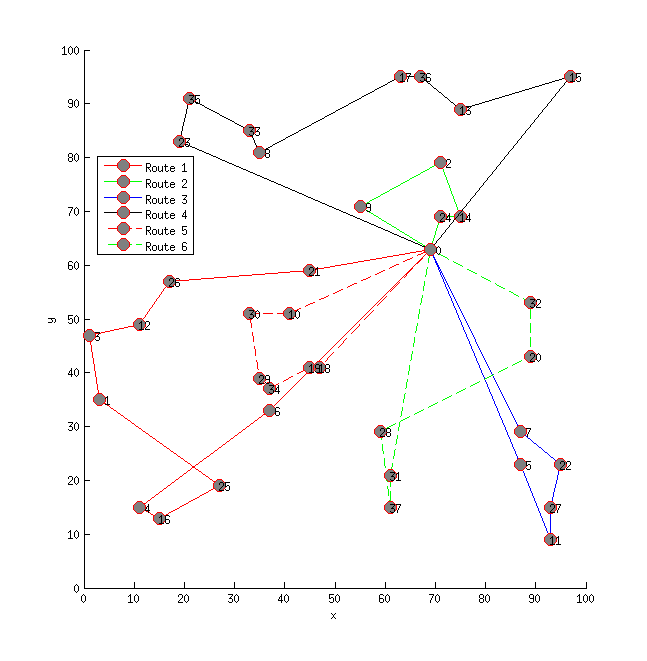
\includegraphics[width=0.45\textwidth] {figures/A-n38-k5-p.png}
        \label{fig:A-n38-k5-p}
    }

    \subfigure[]{
        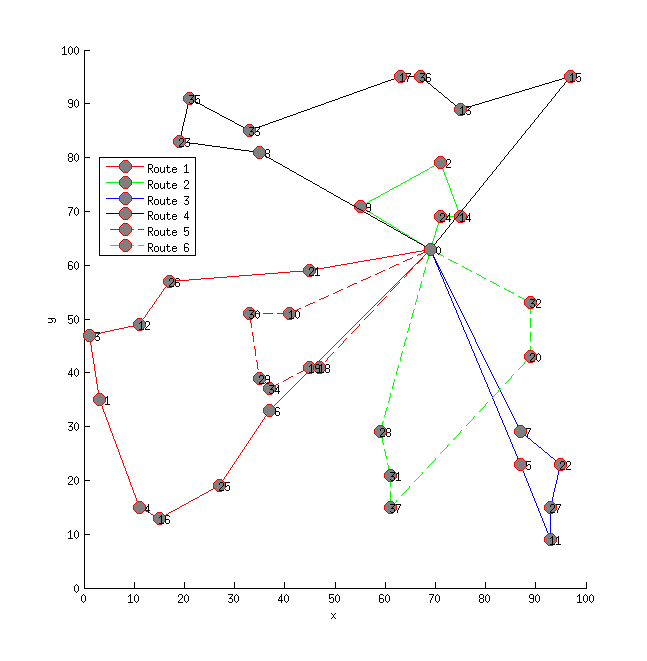
\includegraphics[width=0.45\textwidth] {figures/A-n38-k5-p-2-opt.png}
        \label{fig:A-n38-k5-p-2-opt}
    }

    \cprotect\caption{Graphical depiction of the routes generated 
            by the proposed solution (dataset \verb?A-n38-k5?), (a) after a CWS run 
            (parallel version) and (b) after the 2-opt local search procedure.}
    \label{fig:A-n38-k5-p-graph}

\end{figure}

The closest values to the optimal solutions are obtained for datasets \verb?A-n34-k5? and 
\verb?A-n38-k5?, after 
a 2-opt local search on the solution provided by the parallel version of the 
CWS algorithm (solution value differences of 31 and 55 units, respectively). 
Listings~\ref{lst:routes-opt} and~\ref{lst:routes-own} provide the differences 
between the optimal routes and those found by the proposed CWS constructive 
heuristic \& 2-opt local search combination, for the dataset \verb?A-n38-k5?.\vertbreak

One can identify similarities between some of the routes, 
particularly between Route 4 in Listing~\ref{lst:routes-opt} and Route 1 
in Listing~\ref{lst:routes-own} or between Route 1 and Route 3. This may 
indicate that, in addition to a local search routine that swaps elements within 
individual routes, one may benefit from attempting swaps between different 
routes, such as the $\lambda$-interchange mechanism suggested in~\cite{Osman1993}, and 
which is applied in the SA proposed in Section~\ref{subsec:metaheuristics}. The 
graphical representations of the same routes, given in 
Figure~\ref{fig:A-n38-k5-p-graph} show how the 2-opt local search procedure 
removed crossings between links, specifically Routes 1 and 6, along with an 
enhancement of Route 4, achieved via (1) the swap between nodes 23 and 8 (arcs 
$(0,23) \rightarrow (0,8)$ and $(8,17) \rightarrow (23,17)$) and (2) a swap 
between nodes 33 and 23 (arcs 
$(8,33) \rightarrow (8,23)$ and $(23,17) \rightarrow (33,17)$).\vertbreak

\begin{lstlisting}[label=lst:routes-opt,caption={Optimal routes and solution 
value for the A-n38-k5 dataset. Values provided by Augerat et al.~\cite{website:cvrp-datasets}}]
Route #1: 37 11 27 22 5 7
Route #2: 10 30 29 34 19 18
Route #3: 20 32 15 13 36 17 2 14
Route #4: 28 31 6 25 16 4 1 3 12 26 21
Route #5: 24 33 35 23 8 9
cost 730

\end{lstlisting}

\begin{lstlisting}[label=lst:routes-own,caption={Routes and solution 
value obtained after running the proposed CWS constructive 
heuristic \& 2-opt local search combination, against the dataset A-n38-k5.}]
Route #1: 6 25 16 4 1 3 12 26 21
Route #2: 24 14 2 9
Route #3: 5 11 27 22 7
Route #4: 8 23 35 33 17 36 13 15
Route #5: 10 30 29 34 19 18
Route #6: 28 31 37 20 32
cost 785

\end{lstlisting}

\subsection{Simulated Annealing}
\label{subsec:res-sa}

Following the focus on the example given by dataset \verb?A-n38-k5?, 
Figure~\ref{fig:A-n38-k5-s-sa} shows the graphical results of a SA run, 
starting with the solution given by the sequential version of the CWS algorithm. 
Besides the improvement versus both the sequential and parallel versions of 
the CWS algorithm ($e(.) = 753$ vs. [785, 908]), the joint inspection of 
Listings~\ref{lst:routes-opt} and~\ref{lst:routes-sa} shows how closer the SA 
solution is to the optimal. These results were obtained with the following set 
of parameters for the SA algorithm:

\begin{itemize}

    \item $T_s = 295.75$
    \item $\alpha = 0.005$
    \item $L = 35000$
    \item Stopping condition: 300 iterations without change in $S_c$.

\end{itemize}\vertbreak

\begin{figure}[h!]
    \centering

    \subfigure[]{
        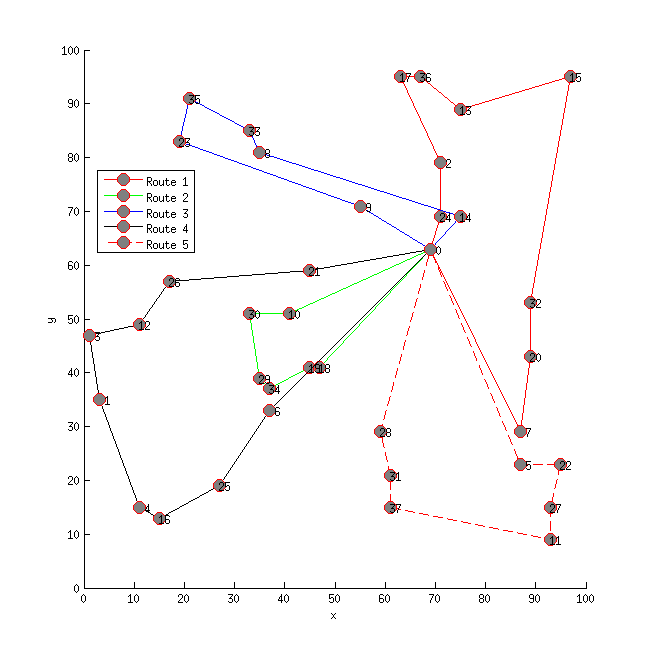
\includegraphics[width=0.45\textwidth] {figures/A-n38-k5-s-sa-graph.png}
        \label{fig:A-n38-k5-s-sa-graph}
    }

    \subfigure[]{
        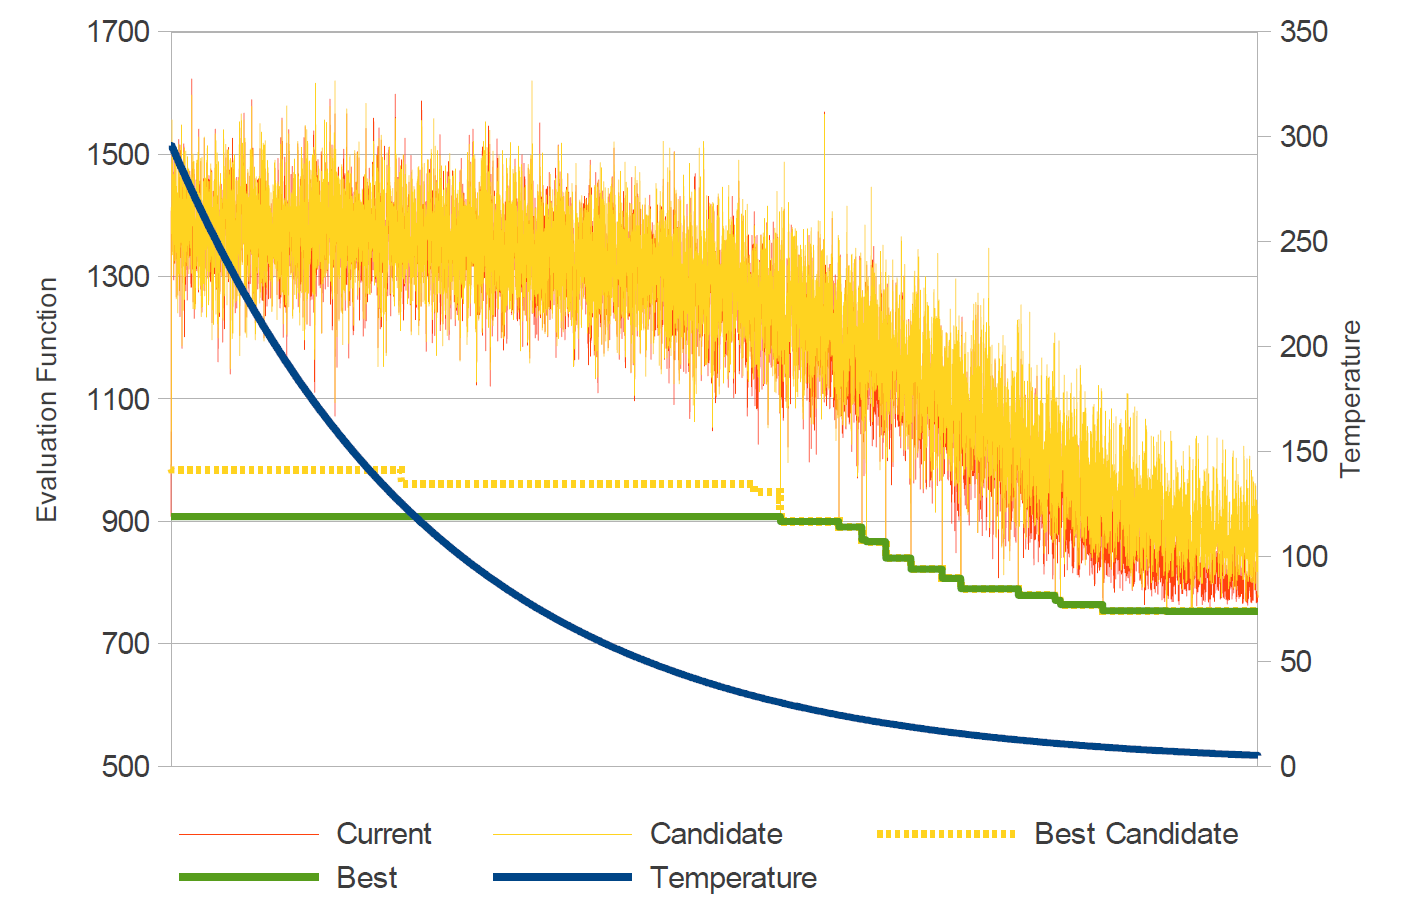
\includegraphics[width=0.45\textwidth] {figures/A-n38-k5-s-sa.png}
        \label{fig:A-n38-k5-s-sa-chart}
    }

    \cprotect\caption{Graphical depiction of the routes generated 
            by the proposed SA implementation (dataset \verb?A-n38-k5?), starting 
            with the solution from the sequential version of the CWS algorithm 
            (a); depiction of the evolution of the SA procedure, with 
            $T_s = 295.75$, $\alpha = 0.005$, $L = 35000$, for a total number of 
            iterations of $27.62$\,M (b).}
    \label{fig:A-n38-k5-s-sa}

\end{figure}

\begin{lstlisting}[label=lst:routes-sa,caption={Routes and solution 
value obtained after running the proposed SA implementation 
metaheuristic, against the dataset A-n38-k5.}]
Route #1: 24 2 17 36 13 15 32 20 7
Route #2: 10 30 29 34 19 18
Route #3: 9 23 35 33 8 14
Route #4: 6 25 16 4 1 3 12 26 21
Route #5: 5 22 27 11 37 31 28
cost 753

\end{lstlisting}

Tables~\ref{tab:sa-results-1} and~\ref{tab:sa-results-2} provide a list of the 
results obtained by the proposed SA implementation, against several of the 
same datasets used in Section~\ref{subsec:res-cws}, with $L = 35000$ (with 
some noted exceptions) and the 
stop criterion being the occurrence of more than 300 iteration without change in 
$S_c$. The results confirm that 
SA techniques are costly in terms of time, while achieving improvements for 
all the datasets, for both versions of the CWS algorithm and the effect of 
changing some of the algorithm parameters (the initial temperature $T_s$ is 
automatically calculated using the method shown 
in~\ref{subsec:cooling}, however an additional test with $10 \times T_s$ was 
performed for each of the datasets chosen for evaluation).\vertbreak

\begin{table}[h!]
    \centering
    \begin{threeparttable}
    \footnotesize
        \begin{tabularx}{0.45\textwidth}{ X X X X X }
            %\hline
            \toprule
            \textbf{Dataset} & $T_s$ & $\alpha$ & $S_i$ & $S_b$ \\ [0.5ex]
            \midrule
            \multirow{4}{*}{A-n38-k5}   & \multirow{2}{*}{295.75}   & 0.005 & \multirow{2}{*}{908}\tnote{1}  & 753   \\ [0.5ex]
                                        &                           & 0.05  &                       & 753   \\ [0.5ex]
            \cmidrule{2-5}
                                        & \multirow{2}{*}{2957.50}  & 0.005 & \multirow{2}{*}{908}\tnote{1}  & 753   \\ [0.5ex]
                                        &                           & 0.05  &                       & 753   \\ [0.5ex]
            \midrule
            \multirow{4}{*}{M-n151-k12} & \multirow{2}{*}{158.70}   & 0.005 & \multirow{2}{*}{1404}\tnote{1} & 1142  \\ [0.5ex]
                                        &                           & 0.05  &                       & 1142  \\ [0.5ex]
            \cmidrule{2-5}
                                        & \multirow{2}{*}{1586.96}  & 0.005 & \multirow{2}{*}{1404}\tnote{1} & 1134  \\ [0.5ex]
                                        &                           & 0.05  &                       & 1128  \\ [0.5ex]
            \cmidrule{2-5}
                                        & 4530.06                   & 0.005 & 1198\tnote{2}                  & 1135  \\ [0.5ex]
            \midrule
            \multirow{4}{*}{M-n200-k17} & \multirow{2}{*}{389.53}   & 0.005 & \multirow{2}{*}{1797}\tnote{1} & 1485  \\ [0.5ex]
                                        &                           & 0.05  &                       & 1442  \\ [0.5ex]
            \cmidrule{2-5}
                                        & \multirow{4}{*}{3895.28}  & 0.005 & \multirow{4}{*}{1797}\tnote{1} & 1461  \\ [0.5ex]
                                        &                           & 0.005 &                       & 1433\tnote{3}  \\ [0.5ex] % 50000
                                        &                           & 0.05  &                       & 1433  \\ [0.5ex]
                                        &                           & 0.05  &                       & 1491\tnote{3}  \\ [0.5ex] % 50000
            \cmidrule{2-5}
                                        & 4270.38                   & 0.005 & 1500\tnote{2}                  & 1470  \\ [0.5ex]
            \bottomrule
        \end{tabularx}
        \begin{tablenotes}
            \footnotesize
            \item[1]Initial solution value after the sequential version of the CWS algorithm.
            \item[2]Initial solution value after the parallel version of the CWS algorithm.
            \item[3]$L = 50000$.
        \end{tablenotes}
    \caption{Results obtained by the proposed SA implementation, against 
            several datasets available in~\cite{website:cvrp-datasets}, and 
            according to different values for $S_i$, $T_s$ and $\alpha$. 
            $L = 35000$ and stop criterion equal to 300 iterations without 
            change in $S_c$, otherwise noted.}
    \label{tab:sa-results-1}
    \end{threeparttable}
    %\end{center}
\end{table}

\begin{table}[h!]
    \centering
    \begin{threeparttable}
    \footnotesize
        \begin{tabularx}{0.45\textwidth}{ l l l l X X }
            %\hline
            \toprule
            \textbf{Dataset} & $T_s$ & $\alpha$ & $S_i$ & $T_{exec}$ & $N_{iter}$ \\ [0.5ex]
            \midrule
            \multirow{4}{*}{A-n38-k5}   & \multirow{2}{*}{295.75}   & 0.005 & \multirow{2}{*}{908}\tnote{1}  & 154.69    & 27.62 M   \\ [0.5ex]
                                        &                           & 0.05  &                       & 17.17     & 3.01 M    \\ [0.5ex]
            \cmidrule{2-6}
                                        & \multirow{2}{*}{2957.50}  & 0.005 & \multirow{2}{*}{908}\tnote{1}  & 226.80    & 43.75 M   \\ [0.5ex]
                                        &                           & 0.05  &                       & 28.72     & 5.22 M    \\ [0.5ex]
            \midrule
            \multirow{4}{*}{M-n151-k12} & \multirow{2}{*}{158.70}   & 0.005 & \multirow{2}{*}{1404}\tnote{1} & 614.72    & 33.71 M   \\ [0.5ex]
                                        &                           & 0.05  &                       & 70.99     & 3.75 M    \\ [0.5ex]
            \cmidrule{2-6}
                                        & \multirow{2}{*}{1586.96}  & 0.005 & \multirow{2}{*}{1404}\tnote{1} & 758.51    & 48.44 M   \\ [0.5ex]
                                        &                           & 0.05  &                       & 85.52     & 5.25 M    \\ [0.5ex]
            \cmidrule{2-6}
                                        & 4530.06                   & 0.005 & 1198\tnote{2}                  & 878.32    & 57.33 M   \\ [0.5ex]
            \midrule
            \multirow{4}{*}{M-n200-k17} & \multirow{2}{*}{389.53}   & 0.005 & \multirow{2}{*}{1797}\tnote{1} & 744.66    & 38.36 M   \\ [0.5ex]
                                        &                           & 0.05  &                       & 86.92     & 4.24 M    \\ [0.5ex]
            \cmidrule{2-6}
                                        & \multirow{4}{*}{3895.28}  & 0.005 & \multirow{4}{*}{1797}\tnote{1} & 918.86    & 55.37 M   \\ [0.5ex]
                                        &                           & 0.005 &                       & 1332.25\tnote{3}   & 79.55 M   \\ [0.5ex] % 50000
                                        &                           & 0.05  &                       & 106.06    & 5.92 M    \\ [0.5ex]
                                        &                           & 0.05  &                       & 131.77\tnote{3}    & 7.9 M     \\ [0.5ex] % 50000
            \cmidrule{2-6}
                                        & 4270.38                   & 0.005 & 1500\tnote{2}                  & 912.66    & 55.20 M   \\ [0.5ex]
            \bottomrule
        \end{tabularx}
        \begin{tablenotes}
            \footnotesize
            \item[1]Initial solution value after the sequential version of the CWS algorithm.
            \item[2]Initial solution value after the parallel version of the CWS algorithm.
            \item[3]$L = 50000$.
        \end{tablenotes}
    \caption{Execution times and iteration numbers obtained by running the 
            proposed SA implementation against 
            several datasets available in~\cite{website:cvrp-datasets}, and 
            according to different values for $S_i$, $T_s$ and $\alpha$. 
            $L = 35000$ and stop criterion equal to 300 iterations without 
            change in $S_c$, otherwise noted.}
    \label{tab:sa-results-2}
    \end{threeparttable}
    %\end{center}
\end{table}

Table~\ref{tab:sa-results-1} shows that for the \verb?A-n38-k5?, with a rather 
small number of stations and routes, the same result of the evaluation function 
is obtained for all variations of SA parameters. Such a result is probably 
caused by the use of the same initial solution already optimized by the CWS 
algorithm and the rather limited 1-interchange local search heuristic used for 
neighbor generation (a 2-interchange mechanism would probably generate better 
results, i.e. better `escapes' from local optima).\vertbreak

For the \verb?M-n151-k12? and 
\verb?M-n200-k17? datasets, the best results are obtained for the largest 
tested $\alpha = 0.05$ (even though one achieves the same best result for the 
\verb?M-n200-k17? --- $e(.) = 1433$ --- with $\alpha = 0.005$ and $L = 50000$) 
which seems somewhat counterintuitive. Due to the stochastic 
nature of the SA approach, such a result is plausible. Nevertheless, it was also 
noted that most of the improvements for the larger datasets occurred during the 
final phases of the algorithm, i.e. in the `colder', `hill-climber' phase of 
the algorithm, which seems to indicate the SA implementation keeps getting 
stuck in the same local optimum. Although the probabilistic nature of the SA 
algorithm should avoid such a situation, this is maybe caused by the use of 
solutions generated by the CWS algorithm (in 
the case of the \verb?M-n151-k12? and \verb?M-n200-k17? datasets those provided 
by the parallel version are also used) and the use of a `poor' 1-interchange 
neighbor generation mechanism.\vertbreak

\subsection{Genetic Algortithm}
\label{subsec:gen-al}

Table~\ref{tab:ga-results-1} summarizes the results obtained with our GA 
implementation, for datasets \verb?A-n38-k5?, \verb?A-n60-k5? and 
\verb?M-n200-k17?. As mentioned in Section~\ref{subsec:ga}, the initial 
populations contain the solutions provided by the CWS algorithm (both parallel 
and sequential versions) as well as that generated via SA, with the following 
parameters:

\begin{itemize}
    \item $T_s = 2957.50$ (\verb?A-n38-k5?), $T_s = 3318.20$ (\verb?A-n60-k5?), $T_s = 3895.28$ (\verb?M-n200-k17?).
    \item $\alpha = 0.05$
    \item $L = 25000$
    \item Stopping condition: 300 iterations without change in $S_c$.
\end{itemize}\vertbreak

The number of generations was set to $G = 10000$ for all experiments summarized 
in Table~\ref{tab:ga-results-1}, and several values for the population size $N$, 
and mutation probability $M$ were used.\vertbreak

\begin{table}[h!]
    \centering
    \begin{threeparttable}
    \footnotesize
        \begin{tabularx}{0.45\textwidth}{ l X X X X X X X}
            %\hline
            \toprule
            \textbf{Dataset} & $N$ & $M$ & $S_i$ & $S_b$ & $G_i$ & $T_{exec}$\\ [0.5ex]
            \midrule
            \multirow{9}{*}{A-n38-k5}   & \multirow{3}{*}{30}   & 0.25  & \textbf{752} & 752 & 0 & 14.29\\ [0.5ex]
                                        &                       & 0.50  & 753 & 753 & 0 & 14.12\\ [0.5ex]
                                        &                       & 0.75  & 753 & 753 & 0 & 14.30\\ [0.5ex]
            \cmidrule{2-7}
                                        & \multirow{3}{*}{60}   & 0.25  & \textbf{752} & 752 & 0 & 27.33\\ [0.5ex]
                                        &                       & 0.50  & 754 & 754 & 0 & 27.36\\ [0.5ex]
                                        &                       & 0.75  & 753 & 753 & 0 & 28.47\\ [0.5ex]
            \cmidrule{2-7}
                                        & \multirow{3}{*}{120}  & 0.25  & 753 & \textbf{752} & 1931 & 56.77\\ [0.5ex]
                                        &                       & 0.50  & 753 & 753 & 0 & 57.11\\ [0.5ex]
                                        &                       & 0.75  & \textbf{752} & 752 & 0 & 57.75\\ [0.5ex]
            \midrule
            \multirow{9}{*}{A-n60-k5}   & \multirow{3}{*}{30}   & 0.25  & \textbf{1381} & 1381 & 0 & 15.88\\ [0.5ex]
                                        &                       & 0.50  & 1387 & 1387 & 0 & 15.92\\ [0.5ex]
                                        &                       & 0.75  & 1389 & 1389 & 0 & 16.27\\ [0.5ex]
            \cmidrule{2-7}
                                        & \multirow{3}{*}{60}   & 0.25  & 1389 & 1389 & 0 & 23.67\\ [0.5ex]
                                        &                       & 0.50  & 1391 & 1391 & 0 & 26.06\\ [0.5ex]
                                        &                       & 0.75  & 1389 & 1389 & 0 & 27.86\\ [0.5ex]
            \cmidrule{2-7}
                                        & \multirow{3}{*}{120}  & 0.25  & 1391 & 1391 & 0 & 51.66\\ [0.5ex]
                                        &                       & 0.50  & 1388 & 1385 & 1175 & 52.94\\ [0.5ex]
                                        &                       & 0.75  & \textbf{1381} & 1381 & 0 & 60.39\\ [0.5ex]
            \midrule
            \multirow{9}{*}{M-n200-k17} & \multirow{3}{*}{30}   & 0.25  & 1446 & 1442 & 3080 & 40.92\\ [0.5ex]
                                        &                       & 0.50  & 1460 & 1456 & 2400 & 42.84\\ [0.5ex]
                                        &                       & 0.75  & 1451 & 1447 & 3168 & 43.26\\ [0.5ex]
            \cmidrule{2-7}
                                        & \multirow{3}{*}{60}   & 0.25  & 1439 & 1439 & 0 & 93.38\\ [0.5ex]
                                        &                       & 0.50  & 1443 & 1443 & 0 & 98.24\\ [0.5ex]
                                        &                       & 0.75  & 1462 & 1451 & 5263 & 102.48\\ [0.5ex]
            \cmidrule{2-7}
                                        & \multirow{3}{*}{120}  & 0.25  & 1452 & 1452 & 0 & 188.37\\ [0.5ex]
                                        &                       & 0.50  & 1435 & \textbf{1429} & 6776 & 177.16\\ [0.5ex]
                                        &                       & 0.75  & 1462 & 1460 & 9448 & 236.99\\ [0.5ex]
            \bottomrule
        \end{tabularx}
        %\begin{tablenotes}
            %\footnotesize
            %\item[1]Initial solution value after the sequential version of the CWS algorithm.
            %\item[2]Initial solution value after the parallel version of the CWS algorithm.
            %\item[3]$L = 50000$.
        %\end{tablenotes}
    \caption{Results obtained by the proposed GA implementation, against 
            several datasets available in~\cite{website:cvrp-datasets}, with 
            $G = 10000$ and variable $N$, $M$. The initial population 
            includes the solutions provided by the previously implemented 
            CWS algorithm (both parallel and sequential versions) and SA method.  
            Includes execution times, $T_{exec}$, in seconds.}
    \label{tab:ga-results-1}
    \end{threeparttable}
    %\end{center}
\end{table}

Overall, the results show that our GA implementation does not yield significant 
benefits when compared with the solutions provided by SA. For most cases, the 
solution generated by the latter method prevails through the $G$ generations. 
With the lowest value of $M$, one also verifies the populations $P(t)$ tend to 
homogeneity, with solution $S_b$ becoming the most common in the successive 
generations $t$, as $t \rightarrow G$. Nevertheless, for the larger dataset, 
\verb?M-n200-k17?, our GA implementation was able to improve the initially 
provided solutions in most of the runs (probably due to `poor' SA solutions 
caused by a low $\alpha$, which provided some room for improvement) and even 
found an overall best solution for this dataset, with value $e(.) = 1429$, with 
parameters $N = 120$, $M = 0.50$ at generation $G_i = 6776$.\vertbreak 

\begin{figure}[h!]
    \centering

    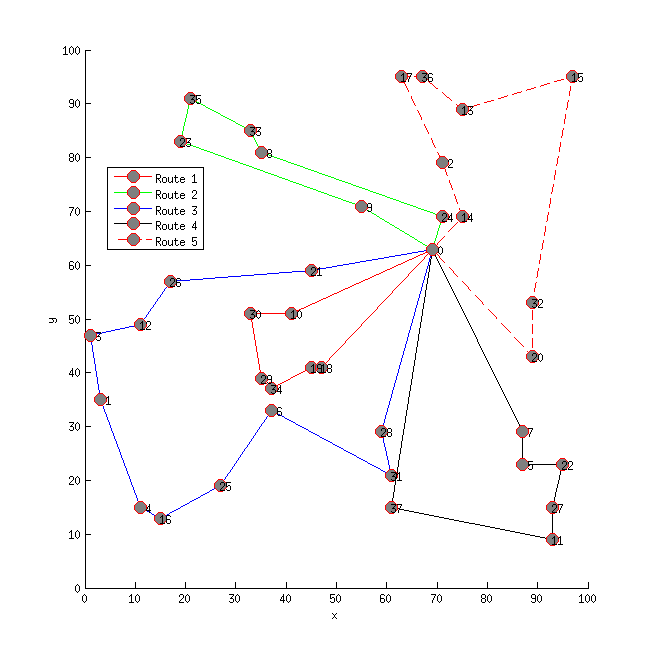
\includegraphics[width=0.45\textwidth] {figures/A-n38-k5-s-ga.png}
    \cprotect\caption{Graphical depiction of the routes generated 
            by the proposed GA implementation (dataset \verb?A-n38-k5?), with 
            parameters $N = 120$ and $M = 0.25$ at generation $G_i = 1931$.}
    \label{fig:A-n38-k5-s-ga-graph}

\end{figure}

\begin{lstlisting}[label=lst:routes-ga,caption={Routes and solution 
value obtained after running the proposed GA implementation, against the 
dataset A-n38-k5.}]
Route #1: 10 30 29 34 19 18
Route #2: 9 23 35 33 8 24
Route #3: 28 31 6 25 16 4 1 3 12 26 21
Route #4: 37 11 27 22 5 7
Route #5: 20 32 15 13 36 17 2 14
cost 752

\end{lstlisting}

During the GA test 
runs, we have also found overall 
best solutions for the \verb?A-n38-k5? dataset, depicted in Figure~\ref{fig:A-n38-k5-s-ga-graph} and 
Listing~\ref{lst:routes-ga} (for $N = 120$, $M = 0.25$, $G_i = 1931$, even though the same 
value had been obtained via SA on previous runs) and the \verb?A-n60-k5? 
dataset, with $e(.) = 1381$ (solution generated via SA).\vertbreak

Following the rather disapointing results shown in Table~\ref{tab:ga-results-1}, 
we have also ran our GA implementation starting with an `unbiased' initial 
population, i.e. without the inclusion of the solutions provided by previously 
implemented methods, only with randomly generated solutions. The results are 
summarized in Table~\ref{tab:ga-results-2}, for $G = 100000$ and $N = 120$, 
which show that the GA implementation is able to produce improvements to the 
initial population, although never as competitive as the CWS or SA methods.\vertbreak

\begin{table}[h!]
    \centering
    \begin{threeparttable}
    \footnotesize
        \begin{tabularx}{0.45\textwidth}{ l X X X X X X X}
            %\hline
            \toprule
            \textbf{Dataset} & $N$ & $M$ & $S_i$ & $S_b$ & $G_i$ & $T_{exec}$\\ [0.5ex]
            \midrule
            \multirow{3}{*}{A-n38-k5}   & \multirow{3}{*}{120}  & 0.25  & 1677 & 788 & 1301     & 38.68\\ [0.5ex]
                                        &                       & 0.50  & 1692 & 773 & 8687     & 46.51\\ [0.5ex]
                                        &                       & 0.75  & 1809 & 834 & 96415    & 51.10\\ [0.5ex]
            \midrule
            \multirow{3}{*}{A-n60-k5}   & \multirow{3}{*}{120}  & 0.25  & 3200 & 1497 & 22855   & 51.03\\ [0.5ex]
                                        &                       & 0.50  & 3195 & 1476 & 22841   & 60.67\\ [0.5ex]
                                        &                       & 0.75  & 3187 & 1458 & 3202    & 63.25\\ [0.5ex]
            \midrule
            \multirow{3}{*}{M-n200-k17} & \multirow{3}{*}{120}  & 0.25  & 6418 & 1558 & 88945   & 194.92\\ [0.5ex]
                                        &                       & 0.50  & 6585 & 1456 & 77971   & 206.74\\ [0.5ex]
                                        &                       & 0.75  & 6540 & 1789 & 49304   & 228.10\\ [0.5ex]
            \bottomrule
        \end{tabularx}
        %\begin{tablenotes}
            %\footnotesize
            %\item[1]Initial solution value after the sequential version of the CWS algorithm.
            %\item[2]Initial solution value after the parallel version of the CWS algorithm.
            %\item[3]$L = 50000$.
        %\end{tablenotes}
    \caption{Results obtained by the proposed GA implementation, against 
            several datasets available in~\cite{website:cvrp-datasets}, with 
            $G = 100000$, $N = 120$ and an initial population entirely composed by 
            randomly generated solutions. 
            Includes execution times, $T_{exec}$, in seconds.}
    \label{tab:ga-results-2}
    \end{threeparttable}
    %\end{center}
\end{table}


